% Created 2021-12-17 Fri 16:54
\documentclass[9pt, b5paper]{article}
\usepackage[UTF8]{ctex}
\usepackage{xltxtra}
\usepackage{bera}
\usepackage[T1]{fontenc}
\usepackage[scaled]{beraserif}
\usepackage[scaled]{berasans}
\usepackage[scaled]{beramono}
\usepackage{graphicx}
\usepackage{xcolor}
\usepackage{multirow}
\usepackage{multicol}
\usepackage{float}
\usepackage{textcomp}
\usepackage{geometry}
\geometry{left=1.2cm,right=1.2cm,top=1.5cm,bottom=1.2cm}
\usepackage{algorithm}
\usepackage{algorithmic}
\usepackage{latexsym}
\usepackage{natbib}
\usepackage{minted}
\newminted{common-lisp}{fontsize=ootnotesize}
\usepackage[xetex,colorlinks=true,CJKbookmarks=true,linkcolor=blue,urlcolor=blue,menucolor=blue]{hyperref}
\author{deepwaterooo}
\date{\today}
\title{安卓中的线程、异步任务、Service与IntentService}
\hypersetup{
  pdfkeywords={},
  pdfsubject={},
  pdfcreator={Emacs 27.1 (Org mode 8.2.7c)}}
\begin{document}

\maketitle
\tableofcontents


\section{Java 创建线程的三种方式总结}
\label{sec-1}
\subsection{继承 Thread 类}
\label{sec-1-1}
\begin{minted}[frame=lines,fontsize=\scriptsize,linenos=false]{java}
class MyThread extends Thread {
    @Override
        public void run() {
        super.run();
    }
}
private void testThread(){
    Thread thread = new MyThread();
    thread.start();
}
\end{minted}
\begin{itemize}
\item 缺点: Java 的单继承限制,想通过 Thread 实现多线程,就只能继承 Thread 类,不可继承其他类。
\end{itemize}
\subsection{实现 Runnable 接口}
\label{sec-1-2}
\begin{itemize}
\item 如果自己的类已经继承了其他类,这时就只能通过实现 Runnable 接口来实现多线程了。
\item 不过,继承 Runnable 接口后,想要启动线程,需要把该类的对象作为参数,传递给 Thread 的构造函数,并使用 Thread 类的实例方法 start 来启动。
\end{itemize}
\begin{minted}[frame=lines,fontsize=\scriptsize,linenos=false]{java}
public class TestThread extends A implements Runnable {
    public void run() {
        // todo
    }
}
// 启动线程
TestThread testThread = new TestThread();
Thread thread = new Thread(testThread);
thread.start();
\end{minted}
\begin{itemize}
\item Thread 内部的 run 方法我们可以看到它的实现原理:
\end{itemize}
\begin{minted}[frame=lines,fontsize=\scriptsize,linenos=false]{java}
private Runnable target;
public void run() {
    if (target != null) {
        target.run();
    }
}
\end{minted}
\begin{itemize}
\item target 是我们传递进来的 Runnable 对象,当线程执行时,线程的 run 方法会直接调用 Runnable 对象的 run 方法。
\end{itemize}
\subsection{实现 Callable 接口}
\label{sec-1-3}
\begin{itemize}
\item 如果想要执行的线程有返回,怎么处理呢?这时应该使用 Callable 接口了,与 Runnable 相比,Callable 可以有返回值,返回值通过 FutureTask 进行封装。
\end{itemize}
\begin{minted}[frame=lines,fontsize=\scriptsize,linenos=false]{java}
public class MyCallable implements Callable<Integer> {
    public Integer call() {
        return 111;
    }
}
public static void main(String[] args) throws ExecutionException, InterruptedException {
    MyCallable mc = new MyCallable();
    FutureTask<Integer> ft = new FutureTask<>(mc);
    Thread thread = new Thread(ft);
    thread.start();
    System.out.println(ft.get());
}
\end{minted}
\subsection{比较}
\label{sec-1-4}
\begin{itemize}
\item 这几种线程创建方式中,实现接口会更好一些,因为:
\begin{itemize}
\item Java 不支持多重继承,因此继承了 Thread 类就无法继承其它类,但是可以实现多个接口。
\item 类可能只要求可执行就行,继承整个 Thread 类开销过大。
\item 另外,如果需要有返回值时,使用 Callable 接口是适合的。
\end{itemize}
\end{itemize}

\section{Handler的使用}
\label{sec-2}
\begin{itemize}
\item Android中,不允许应用程序在子线程中更新UI,UI的处理必须在UI线程中进行,这样Android定制了一套完善的线程间通信机制——Handler通信机制。Handler作为Android线程通信方式,高频率的出现在我们的日常开发工作中,我们常用的场景包括:使用异步线程进行网络通信、后台任务处理等,Handler则负责异步线程与UI线程(主线程)之间的交互。
\item Android为了确保UI操作的线程安全,规定所有的UI操作都必须在主线程(UI线程)中执行,决定了UI线程中不能进行耗时任务,在开发过程中,需要将网络,IO等耗时任务放在工作线程中执行,工作线程中执行完成后需要在UI线程中进行刷新,因此就有了Handler进程内线程通信机制,当然Handler并不是只能用在UI线程与工作线程间的切换,Android中任何线程间通信都可以使用Handler机制。
\end{itemize}
\subsection{UI线程中使用Handler}
\label{sec-2-1}
\begin{itemize}
\item UI线程中使用Handler非常简单,因为框架已经帮我们初始化好了Looper,只需要创建一个Handler对象即可,之后便可以直接使用这个Handler实例向UI线程发消息(子线程--->UI线程)
\end{itemize}
\begin{minted}[frame=lines,fontsize=\scriptsize,linenos=false]{java}
    private Handler handler = new Handler(){
        @Override
        public void handleMessage(@NonNull Message msg) {
            super.handleMessage(msg);
            //处理消息
        }
    };
    @Override
    protected void onCreate(@Nullable Bundle savedInstanceState) {
        super.onCreate(savedInstanceState);
        setContentView(R.layout.activity_six);
    }
\end{minted}
\begin{itemize}
\item 这种方式会导致 \uline{内存泄露} 。
\begin{itemize}
\item 我们通过Handler发送消息,在Message对象中会持有当前Handler对象的引用,在Java中非静态成员类、内部类、匿名类会持有外部对象的引用(这里在源码中有提到),而Looper是线程局部变量,其生命周期与UI线程相同,Looper持有MessageQueue的引用,MessageQueue持有Message的引用,当通过Handler发送一个延时消息未处理之前用户已经离开当前Activity,会导致Activity不能及时释放而内存泄漏。
\end{itemize}
\end{itemize}
\subsubsection{解决思路}
\label{sec-2-1-1}
\begin{enumerate}
\item 官方推荐的一种
\label{sec-2-1-1-1}
\begin{minted}[frame=lines,fontsize=\scriptsize,linenos=false]{java}
private Handler handler = new Handler(new Handler.Callback() {
        @Override
        public boolean handleMessage(@NonNull Message msg) {
            switch (msg.what){
            case 1:
            //处理子线程发过来的消息
            Toast.makeText(SixActivity.this,(String)msg.obj,Toast.LENGTH_LONG).show();
            Log.d("aa",(String) msg.obj);
            break;

            }
            return false;
        }
    });
\end{minted}
\item 静态内部类
\label{sec-2-1-1-2}
\begin{itemize}
\item 下面的例子实现了子线程(执行run()耗时函数的线程)向主线程发送消息
\begin{minted}[frame=lines,fontsize=\scriptsize,linenos=false]{java}
public static final int LOAD_COM = 1; // 加载任务的id标志

private Handler mHandler = new MyHandler(MainActivity.this); // 在MainActivity中,创建了一个Handler对象。

private static class MyHandler extends Handler { // MainActivity中的静态static内部类
    private final WeakReference<MainActivity> mActivity; // 持有当前MainActivity的WeakReference
    private MyHandler(MainActivity activity) {
        this.mActivity = new WeakReference(activity);
    }
    @Override public void handleMessage(@NonNull Message msg) { // ui线程中,负责消息返回的处理逻辑
        super.handleMessage(msg);      // UI线程中,Handler对象的handleMessage方法负责处理消息的返回
        switch (msg.what){
        case LOAD_COM:
            Log.d("TestHandler", msg.obj.toString());
            MainActivity mainActivity = mActivity.get();
            if (mainActivity != null){
                mainActivity.mTextView.setText(msg.obj.toString());
            }
            break;
        }
    }
};
@Override public void onClick(View v) {
    switch (v.getId()) {
    case R.id.start_load: // 当按钮start_load点击时,启动一个后台线程,模拟一个后台加载过程(线程休眠1秒)
        new Thread() {
            @Override
            public void run() { // 后台线程中执行的逻辑:这里代码写定义在主线程MainActivity中,但实际run()函数的真正执行是执行在子线程中
                try {
                    Thread.sleep(1000);
                } catch (InterruptedException e) {
                    e.printStackTrace();
                }
// 子线程发送消息
                // Message message = new Message();//可以使用new Message来创建消息,但是一般不这样使用?
                Message message = Message.obtain(); // 后台任务完成后,使用Handler对象的sendMessage方法发送消息(一个Messaage对象)给UI线程
                message.what = LOAD_COM;
                message.obj = "我是子线程消息";
                mHandler.sendMessage(message); // 从后台线程中,发送消息给UI线程
            }
        }.start();
        break;
    }
}
\end{minted}
\item 主线程给子线程发送消息(UI线程--->子线程)
\begin{minted}[frame=lines,fontsize=\scriptsize,linenos=false]{java}
public class SixActivity extends AppCompatActivity {
    private Handler handler;
    private Button btn;
    @Override
        protected void onCreate(@Nullable Bundle savedInstanceState) {
        super.onCreate(savedInstanceState);
        setContentView(R.layout.activity_six);
        new MyOneThread().start();     // 子线程创建方式
        btn= findViewById(R.id.dian);
        btn.setOnClickListener(new View.OnClickListener() {
                @Override
                    public void onClick(View v) {
                    Message message=Message.obtain();
                    message.what=1;
                    message.obj="我是主线程的消息发送给子线程";
                    handler.sendMessage(message); // 封装完数据发送给子线程
                }
            });
    }
    class MyOneThread extends Thread{
        @Override public void run() {
            // 在子线程中处理消息,子线程中处理消息,没有默认的Loop
            // 由于只有主线程成才默认的Looper.prepare(), Looper.loop();
            Looper.prepare(); // 创建Looper: 如果不添加会报错
            handler = new Handler() { // 在子线程中创建消息Handler
                @Override
                public void handleMessage(@NonNull Message msg) {
                    switch (msg.what){
                    case 1:
                    Log.d("aa",(String) msg.obj);
                    break;
                    }
                }
            };
            // 循环读取messageQueue
            Looper.loop(); // 如果不添加读取不到消息
        }
    }
}
\end{minted}
\item 子线程中,也可以使用这个方式来获取Looper
\end{itemize}
\begin{minted}[frame=lines,fontsize=\scriptsize,linenos=false]{java}
handler = new Handler(Looper.getMainLooper()) {
    @Override
    public void handleMessage(@NonNull Message msg) {
        switch (msg.what) {
        case 1:
        Log.d("aa",(String) msg.obj);
        break;
        }
    }
};
\end{minted}
\begin{itemize}
\item 子线程发送消息到子线程(子线程----->子线程)
\end{itemize}
\begin{minted}[frame=lines,fontsize=\scriptsize,linenos=false]{java}
btn.setOnClickListener(new View.OnClickListener() {
        @Override public void onClick(View v) {
            new Thread(new Runnable() {
                    @Override
                    public void run() {
                        Message message = Message.obtain();
                        message.obj = "我是子线程发送到子线消息";
                        message.what = 1;
                        handler.sendMessage(message); // 发送消息的子线程也是有handler的
                    }
                }).start();
        }
    });
class MyOneThread extends Thread {
    @Override public void run() {
        //在子线程中处理消息,子线程中处理消息,没有默认的Loop
        //由于只有主线程成才默认的Looper.prepare(), Looper.loop();
        // Looper.prepare(); // 创建Looper: 效果一样,换下面的方式
        handler = new Handler(Looper.getMainLooper()){
            @Override
            public void handleMessage(@NonNull Message msg) {
                switch (msg.what){
                case 1:
                Log.d("aa",(String) msg.obj);
                break;
                }
            }
        };
        // Looper.loop(); // 循环读取messageQueue
    }
}
\end{minted}
\begin{itemize}
\item 使用Handler.post()直接更新ui
\end{itemize}
\begin{minted}[frame=lines,fontsize=\scriptsize,linenos=false]{java}
private Handler handler=new Handler();
@Override
protected void onCreate(@Nullable Bundle savedInstanceState) {
    super.onCreate(savedInstanceState);
    setContentView(R.layout.activity_six);
    btn = findViewById(R.id.dian);
    new Thread(new Runnable() {
            @Override
            public void run() {
                // Message message=Message.obtain();
                // message.obj="我是子线程静态消息";
                // message.what=1;
                // handler.sendMessage(message);
                handler.post(new Runnable() {
                        @Override
                        public void run() {
                            Log.d("aa","直接更新Ui");
                            btn.setText("我是更新的消息");
                        }
                    });
            }
        }).start();
}
\end{minted}
\begin{itemize}
\item post和sendMessage本质上是没有区别的,只是实际用法中有一点差别
\item post也没有独特的作用,post本质上还是用sendMessage实现的,post只是一中更方便的用法而已
\end{itemize}

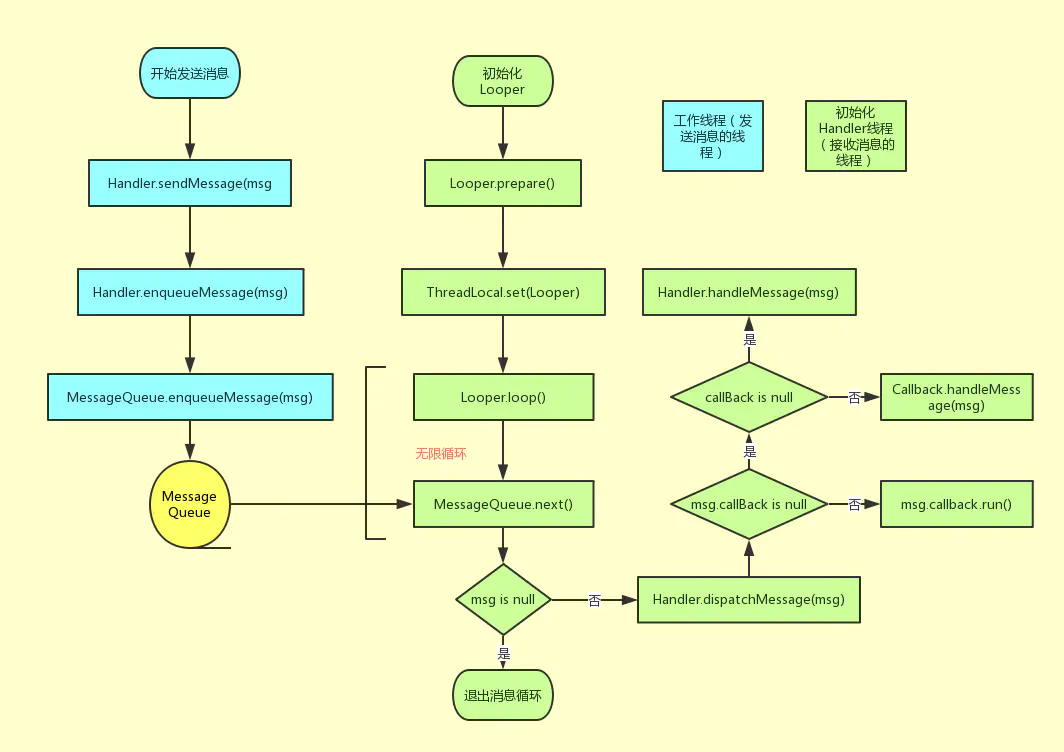
\includegraphics[width=.9\linewidth]{./pic/handler.png}
\end{enumerate}

\subsection{关于安卓handler的面试小问题}
\label{sec-2-2}
\subsubsection{Looper和Handler一定要处于一个线程吗?子线程中可以用MainLooper去创建Handler吗?}
\label{sec-2-2-1}
\begin{itemize}
\item (1)子线程中
\end{itemize}
\begin{minted}[frame=lines,fontsize=\scriptsize,linenos=false]{java}
Handler handler = new Handler(Looper.getMainLooper()); // 此时,子线程的handler与Looper.getMainLooper()主线程Looper, 两者就不在一个线程中
\end{minted}
\begin{itemize}
\item 此时两者就不在一个线程中
\item (2)子线程中可以用MainLooper去创建Handler.
\end{itemize}
\subsubsection{Handler的post方法发送的是同步消息吗?可以发送异步消息吗?}
\label{sec-2-2-2}
\begin{itemize}
\item 用户层面发送的都是同步消息
\item 不能发送异步消息
\item 异步消息只能由系统发送。
\end{itemize}
\subsubsection{Handler.post的逻辑在哪个线程执行的,是由Looper所在线程还是Handler所在线程决定的?}
\label{sec-2-2-3}
\begin{itemize}
\item 由Looper所在线程决定的
\item 最终逻辑是在Looper.loop()方法中,从MsgQueue中拿出msg,并且执行其逻辑,这是在Looper中执行的,因此是由Looper所在的线程决定的。
\end{itemize}
\subsubsection{Handler构造方法中通过Looper.myLooper();是如何获取到当前线程的Looper的?}
\label{sec-2-2-4}
\begin{itemize}
\item myLooper()内部使用ThreadLocal实现,因此能够获取各个线程自己的Looper
\end{itemize}
\subsubsection{MessageQueue(消息队列)}
\label{sec-2-2-5}
\begin{itemize}
\item 消息队列被封装到Looper里面了,我们一般不会直接与MessageQueue打交道。我们只需要记住它是用来存放消息的单链表结构。队列的顺序由Message的next属性来维护。MessageQueue是整个Handler机制的核心,里面涉及很多特性我们这里都不展开讲述(比如消息屏障机制)。
\end{itemize}
\subsection{handler工作原理总结: Handler的工作原理}
\label{sec-2-3}
\begin{itemize}
\item Handler的消息传递机制涉及到四个部分:
\begin{itemize}
\item 1. Message:线程间传递的对象。
\item 2. MessageQueue: 消息队列,用来存放Handler发布的Message.
\item 3. Handler:负责将Message插入到MessageQueue中以及对MessageQueue中的Message进行处理。
\item 4. Looper:负责从MessageQueue中取出Message,并交给Handler.
\end{itemize}
\item 其中:
\begin{itemize}
\item Looper存储在ThreadLocal中,Looper在创建时会同时创建MessageQueue,作为其成员对象.因此Looper和MessageQueue是属于创建者线程的,各线程之间的Looper和MessageQueue相互独立。
\item Handler在创建时会从当前线程的ThreadLocal中取得Looper.
\item 发送消息时,在发送线程中调用接收线程中的Handler的sendMessage方法,过程中,Handler会将自身赋予到Message的target中,并将Message插入到Handler对应的MessageQueue中。
\item 而接收线程中的Looper在循环过程中会取出这个Message,通过Message.target取出接收线程中的Handler,并将消息交Handler对象处理。由此实现了跨线程通信。
\item 要注意的是:线程与Looper和MessageQueue是一对一的关系,即一个线程只维护一个Looper和一个MessageQueue;而线程与Handler的关系是一对多,即一个线程可以有很多Handler,一个Handler只对应一个线程,这也是为什么Handler在发送消息时,为什么要将自身赋给Message.target的原因。
\end{itemize}
\item Handler内存泄露的解决方法
\begin{itemize}
\item 方法1:通过程序逻辑进行保护。
\begin{itemize}
\item 关闭Activity的时候停掉后台线程,这样就相当于切断了Handler和外部连接的线,Activity自然会在合适的时候被回收。
\item 如果你的Handler是被delay的Message持有了引用,那么在Activity销毁前使用相应的Handler的removeCallbacksAndMessages()方法,把消息对象从消息队列移除就行了。
\end{itemize}
\item 方法2:将Handler声明为静态类
\begin{itemize}
\item 静态类不持有外部类的对象,这样即使Handler在运行,Activity也可以被回收。
\item 由于静态类的Handler不再持有外部类对象,如果要操作Activity需要增加一个Activity的弱引用。
\end{itemize}
\end{itemize}
\end{itemize}
% Emacs 27.1 (Org mode 8.2.7c)
\end{document}